\documentclass[a4paper,12pt]{article}
\usepackage[T2A]{fontenc}
\usepackage[utf8]{inputenc}
\usepackage[russian]{babel}
\usepackage{graphicx}
\usepackage{float}
\usepackage{subcaption}
\usepackage{amsmath, amssymb}
\usepackage{geometry}
\usepackage{amsmath}
\usepackage{tikz}
\usepackage{hyperref}
\geometry{top=2cm, bottom=2cm, left=3cm, right=1.5cm}

\begin{document}

\thispagestyle{empty}
\begin{center}
    \large
    Министерство науки и высшего образования Российской Федерации\\
    Федеральное государственное автономное образовательное учреждение\\
    высшего образования\\
    «Национальный исследовательский университет ИТМО»\\
    \vspace{5cm}
    \textbf{Отчёт по исследовательской работе № 1}\\
    \textbf{По предмету: Математический анализ и основы вычислений}\\
    \vspace{6cm}
    \begin{flushright}
        Выполнил работу:\\ Тиганов Вадим Игоревич\\
        \vspace{1cm}
        Академическая группа: \\ J3112\\
        \vspace{1cm}
        Вариант: \\18
    \end{flushright}
    \vspace{1cm}
    \vspace{3cm}
    \begin{center}
        Санкт-Петербург, 2025\\
    \end{center}
\end{center}

\newpage


\section{Ход работы}


\subsection{Задание 8}

Дана функция \(f(x) = \cos^2(x)\) на промежутке \([a,b] = [0, \pi]\)

\section*{Условие задачи}

\subsection*{Аналитический этап}
В рамках данного задания необходимо:

\begin{enumerate}
    \item Составить верхнюю и нижнюю суммы Дарбу, вычислить эти суммы. При необходимости разбивать функцию на участки монотонности.
    
    \item Проверить критерий Римана интегрируемости функции.
    
    \item Найти интегралы Дарбу и сделать вывод об интегрируемости функции, в том числе о значении интеграла.
    
    \item Подобрать еще одно достаточное условие интегрируемости данной функции, отличное от упомянутых критериев и проверить его.
    
    \item Сравнить найденное значение интеграла с ответом по формуле Ньютона-Лейбница.
\end{enumerate}


\emph{Решение задачи:}

\begin{figure}[H]
    \centering
    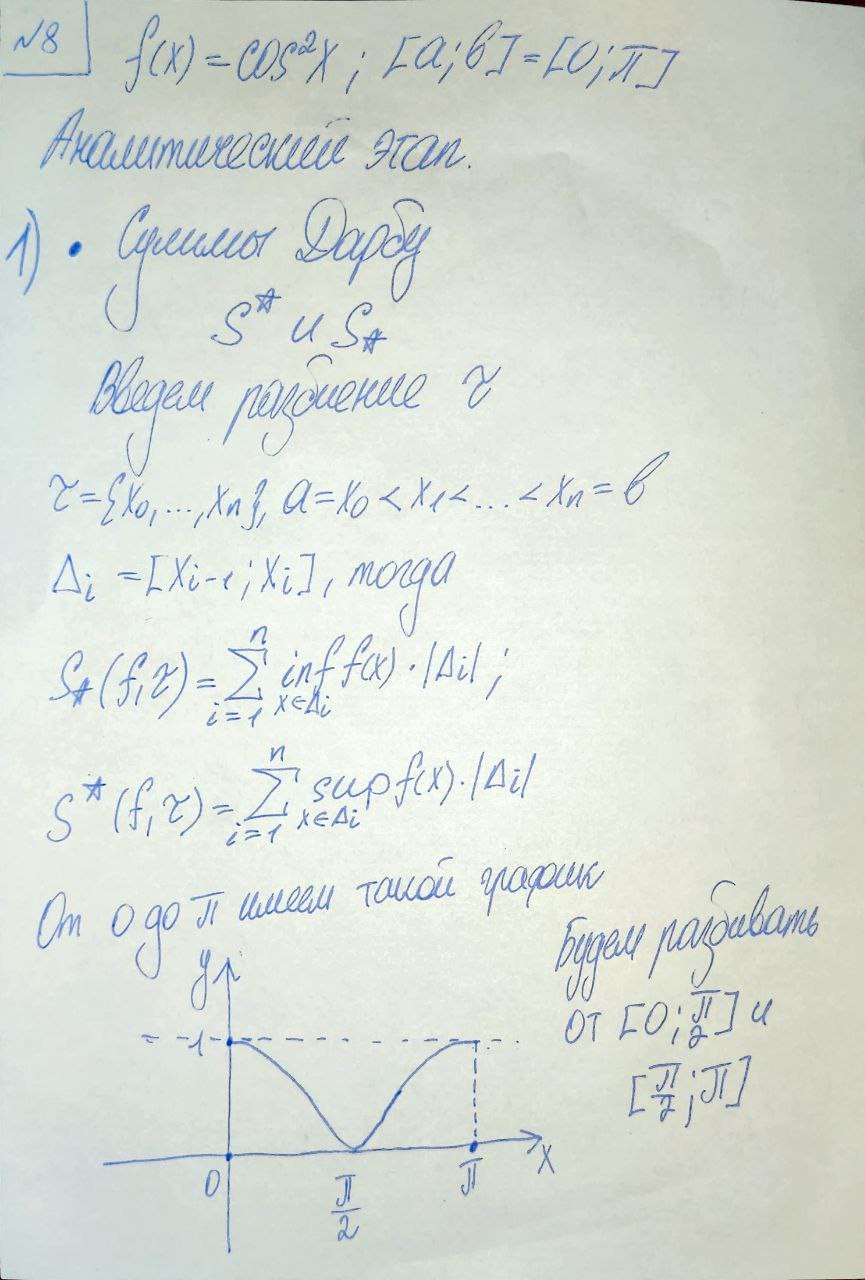
\includegraphics[width=0.8\linewidth]{/home/vadim/Edu/calculus_s2_work1/docs/img/8_1.jpg}
    \label{fig:integral}
\end{figure}

\begin{figure}[H]
    \centering
    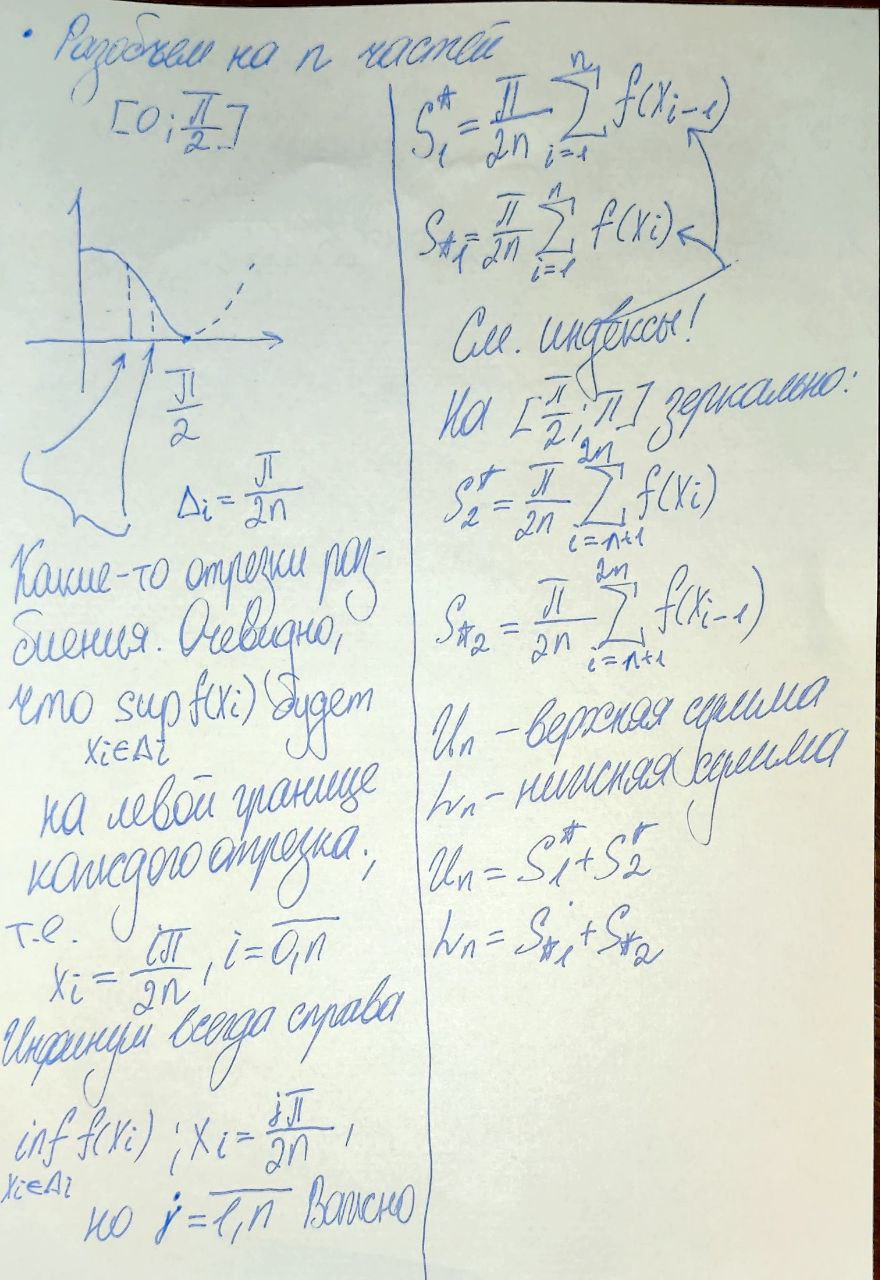
\includegraphics[width=0.8\linewidth]{/home/vadim/Edu/calculus_s2_work1/docs/img/8_2.jpg}
    \label{fig:integral}
\end{figure}

\begin{figure}[H]
    \centering
    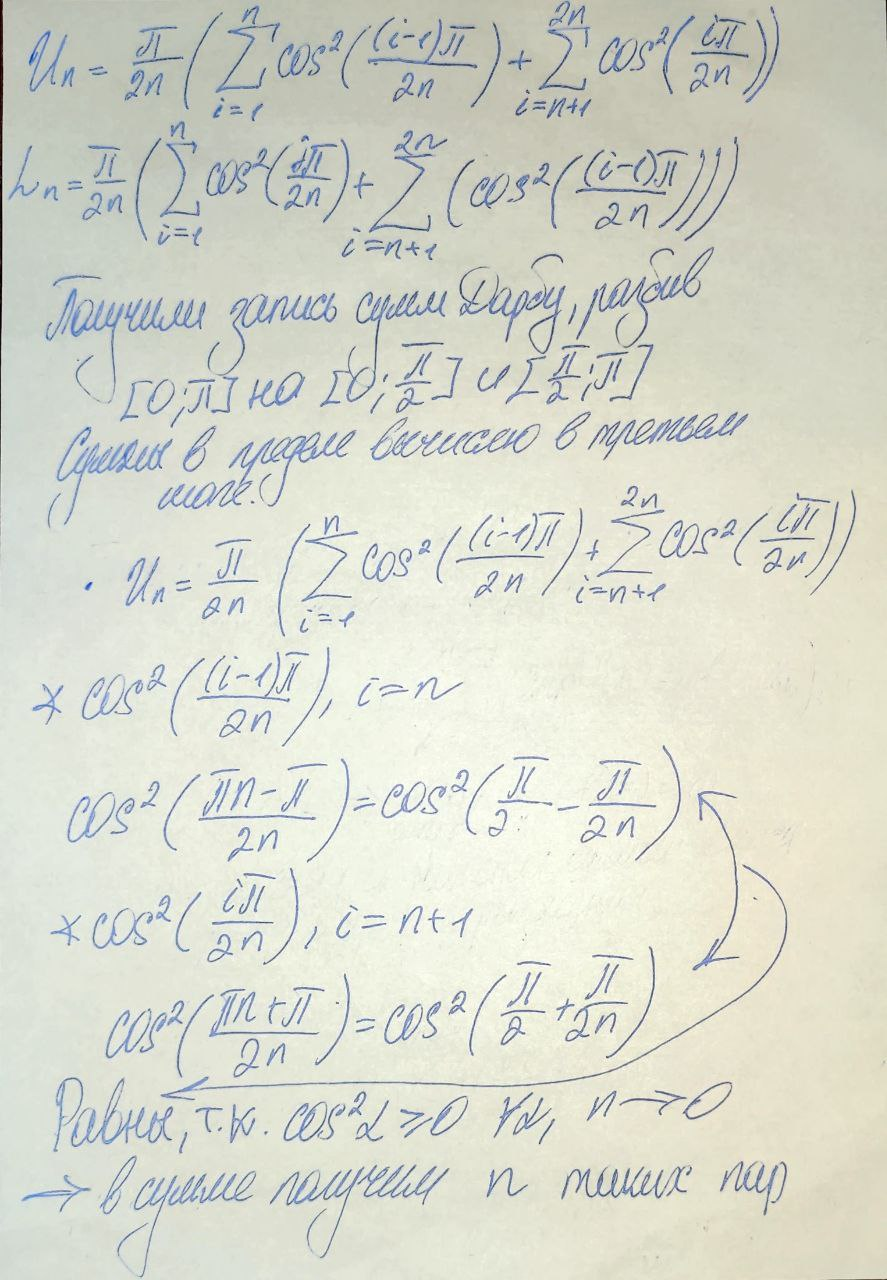
\includegraphics[width=0.8\linewidth]{/home/vadim/Edu/calculus_s2_work1/docs/img/8_3.jpg}
    \label{fig:integral}
\end{figure}

\begin{figure}[H]
    \centering
    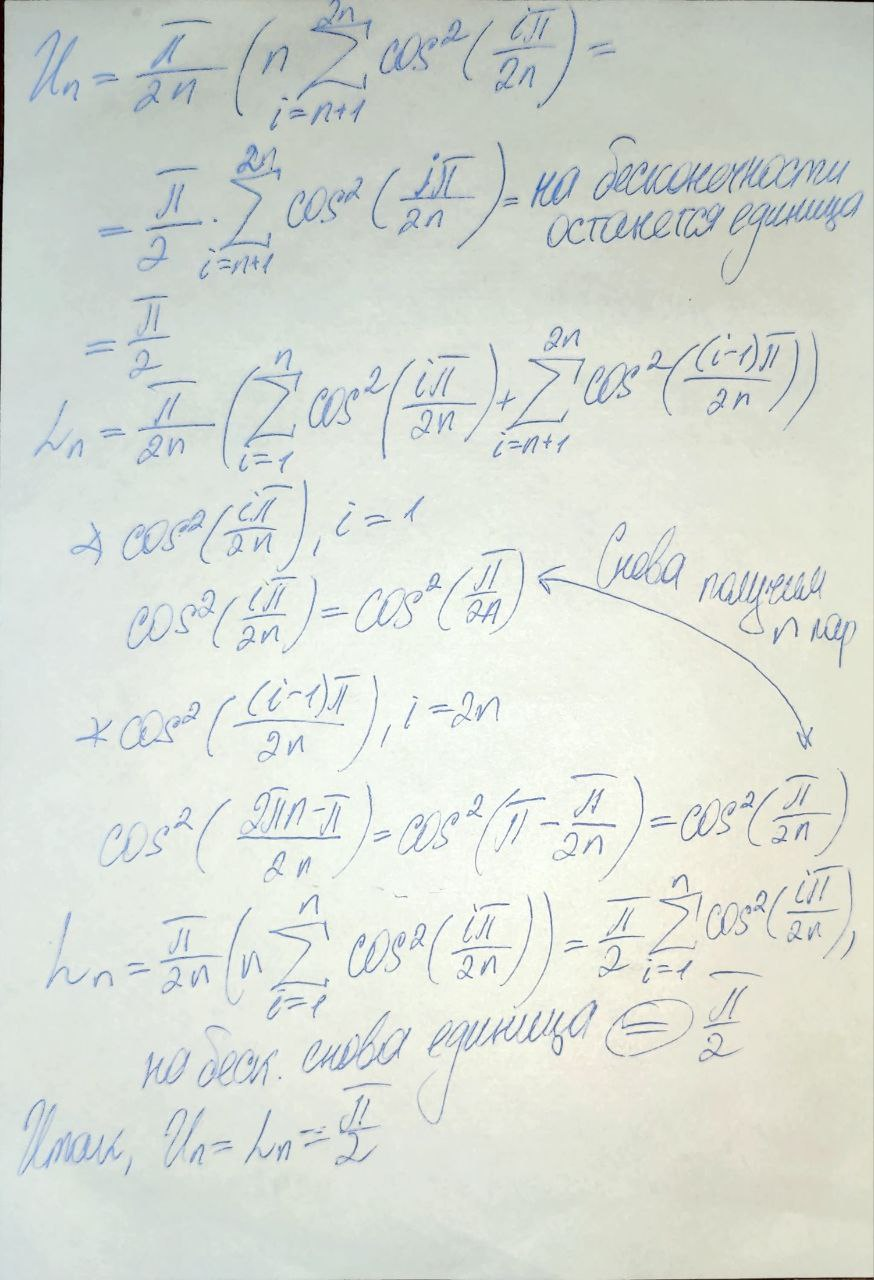
\includegraphics[width=0.8\linewidth]{/home/vadim/Edu/calculus_s2_work1/docs/img/8_4.jpg}
    \label{fig:integral}
\end{figure}

\begin{figure}[H]
    \centering
    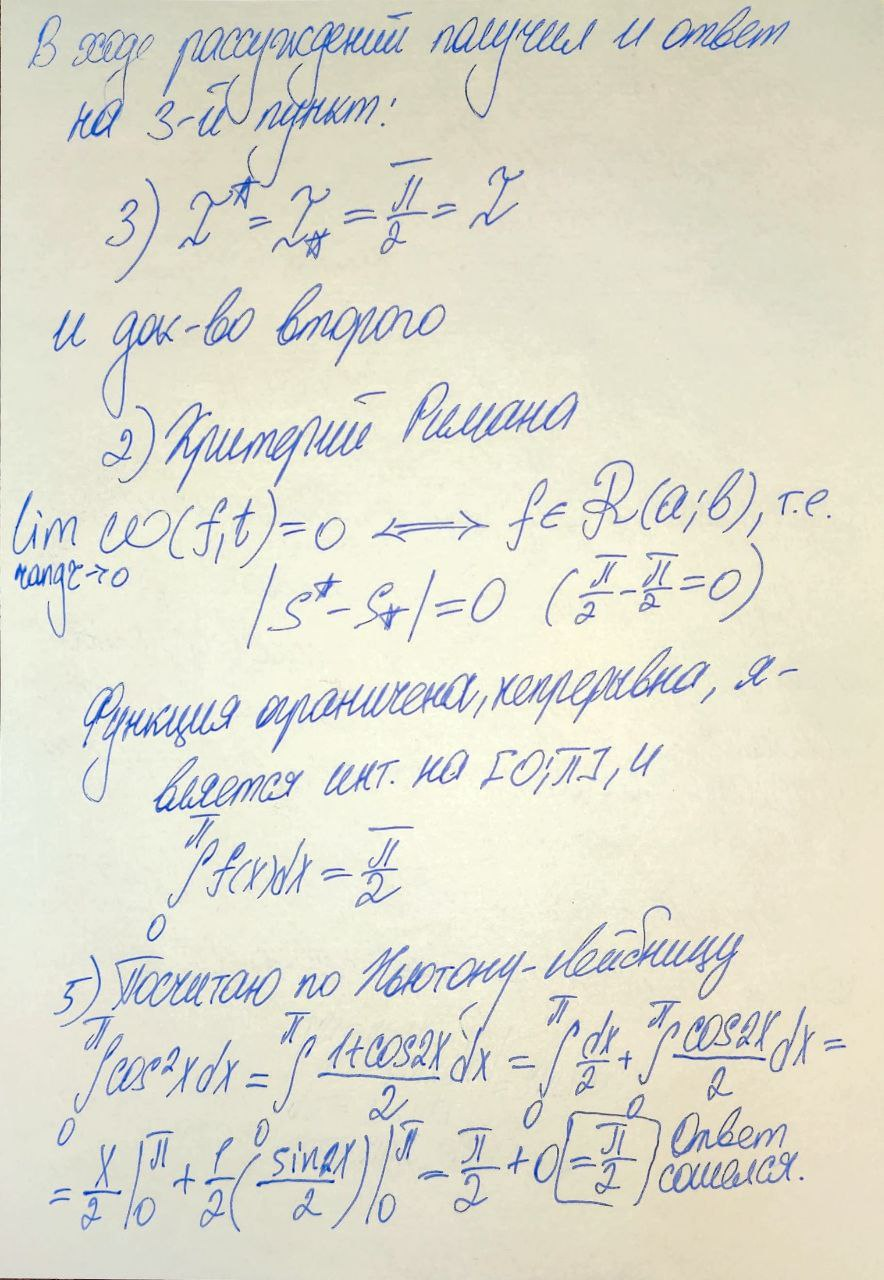
\includegraphics[width=0.8\linewidth]{/home/vadim/Edu/calculus_s2_work1/docs/img/8_5.jpg}
    \label{fig:integral}
\end{figure}

\begin{figure}[H]
    \centering
    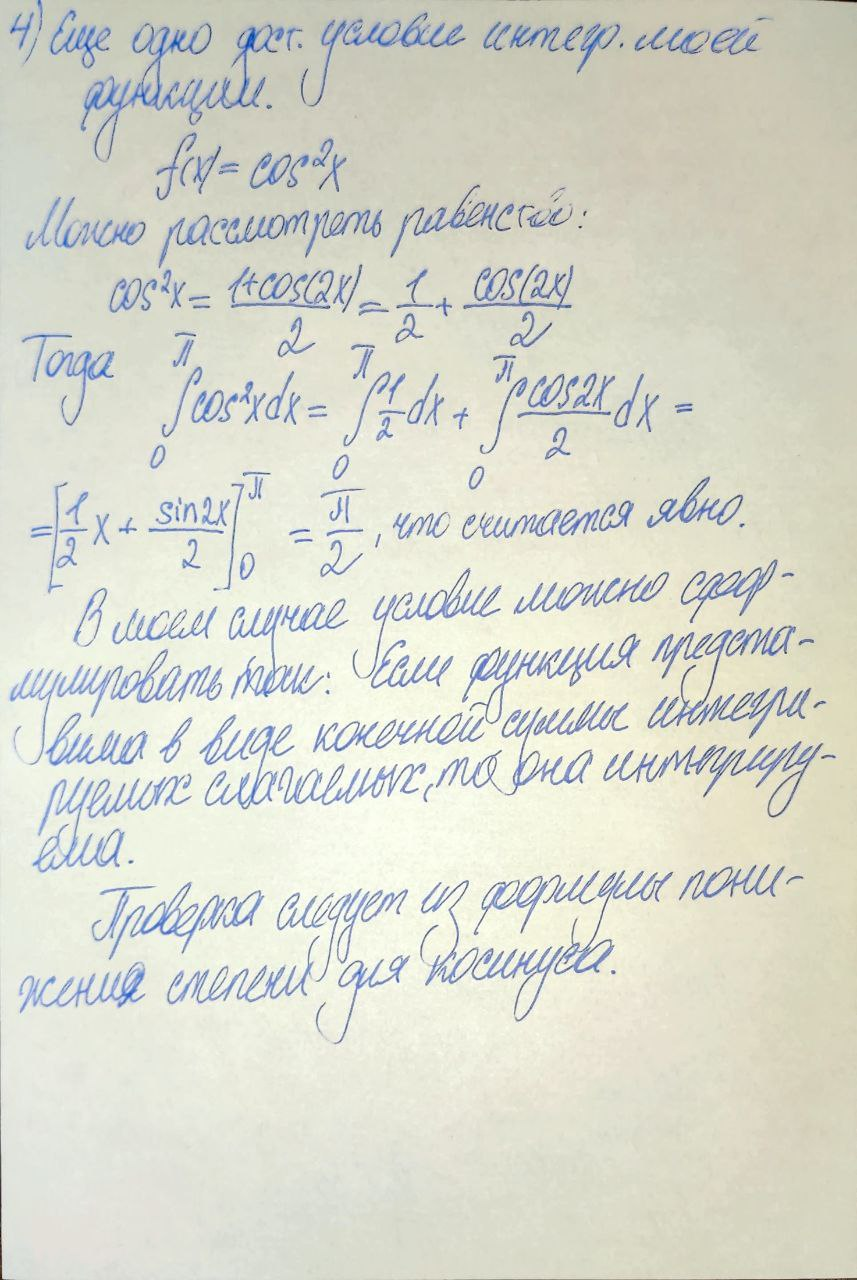
\includegraphics[width=0.8\linewidth]{/home/vadim/Edu/calculus_s2_work1/docs/img/8_6.jpg}
    \label{fig:integral}
\end{figure}

\emph{Ссылка на решение практического этапа работы:}
\href{https://github.com/VTiganov/calculus_s2_work1/blob/main/src/task8/main.ipynb}{link (clickable)}

\end{document}